\section{Systembeskrivelse}
Denne sektion vil beskrive hvordan systemet sat op. samt hvilke chips og boards der er udleveret.
Til projektet er der anvendt det tildelte pan tilt system som har påmonteret 2 hall sensorer samt 2 h-broer som styrer motorerne, der sidder på hhv pan og tilt.\\
Til at styre denne opstilling er der udleveret èt stk Field Programmable Gate Array (FPGA) og èn Micro processor unit (MPU).
\\
%På FPGA'en \cite{Nexys2Datasheet} er der 4 knapper, 8 switches, og 4 7-segment displays som bliver anvendt i projektet.
\subsection{Micro Processor Unit}
Det udleverede Launchpad board fra Texas Instruments har en påmonteret MPU fra Texas Instruments, den udleverede model er en TM4C123GH6PM Arm Cortex M4 \cite{TM4C123GH6PMDatasheet}.\\
Launchpad boardet får strøm gennem micro usb porten som sidder i øverste venstre hjørne som ses på figur \ref{fig:TivaLaunchPad}.\\
Micro usb porten bruges samtidig til at programmere boarded ved hjælp af et Integrated development environment (IDE) til dette projekt blev Code Composer Studio \textsuperscript{\texttrademark} anvendt som er Texas Instruments egen IDE.

\begin{figure}[!ht]
	\begin{center}
		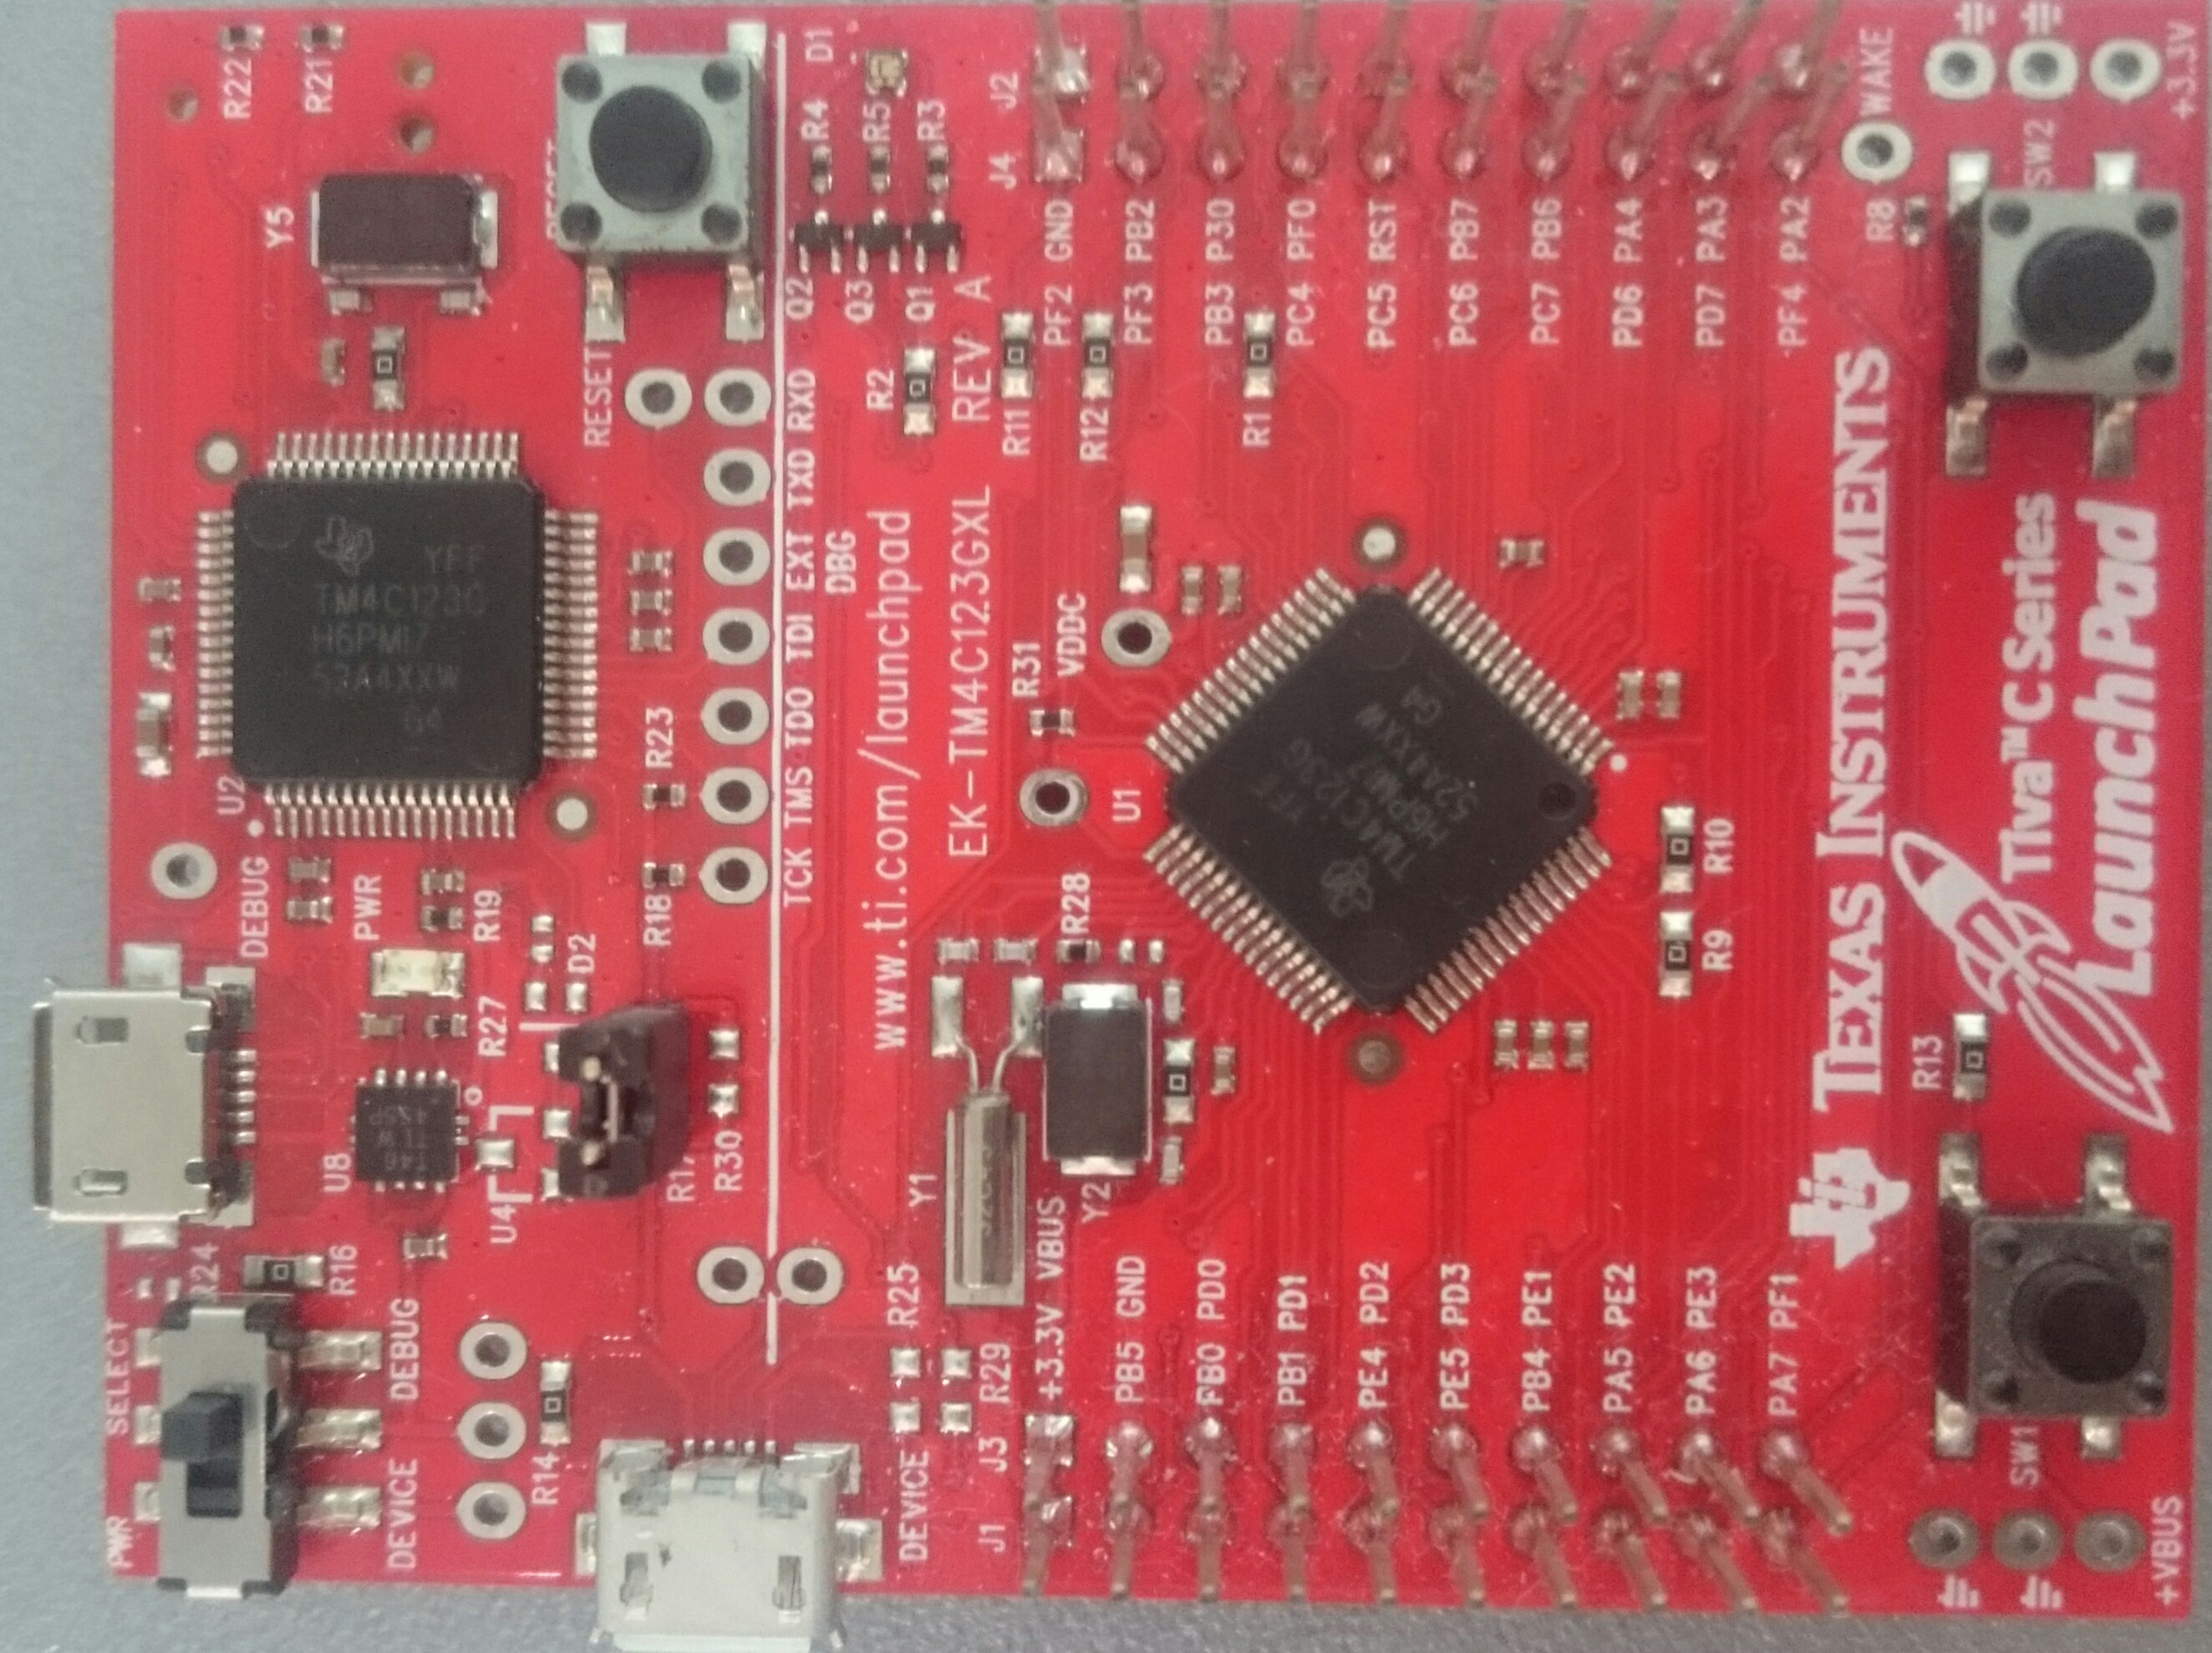
\includegraphics[scale=0.1, angle =270]{Billeder/TivaLaunchPad.JPG}
	\end{center}
\caption{Tiva\textsuperscript{\texttrademark} Launchpad boardet med den tilføjede TM4C123GH6PM arm cortex M4 Micro Processor Unit}
\label{fig:TivaLaunchPad}
\end{figure}

Launchpad boarded kan tilføjes til et embedded programmerings board som blev udleveret i starten af semesteret som inkluderer et keypad, et lcd og en drehimpulsgeber, samt en SPI udgang som anvendes til projektet, se figur \ref{fig:EMP_BOARD} og se vedlagt USB disk for datablad, under dokumenter.

\begin{figure}[!ht]
	\begin{center}
		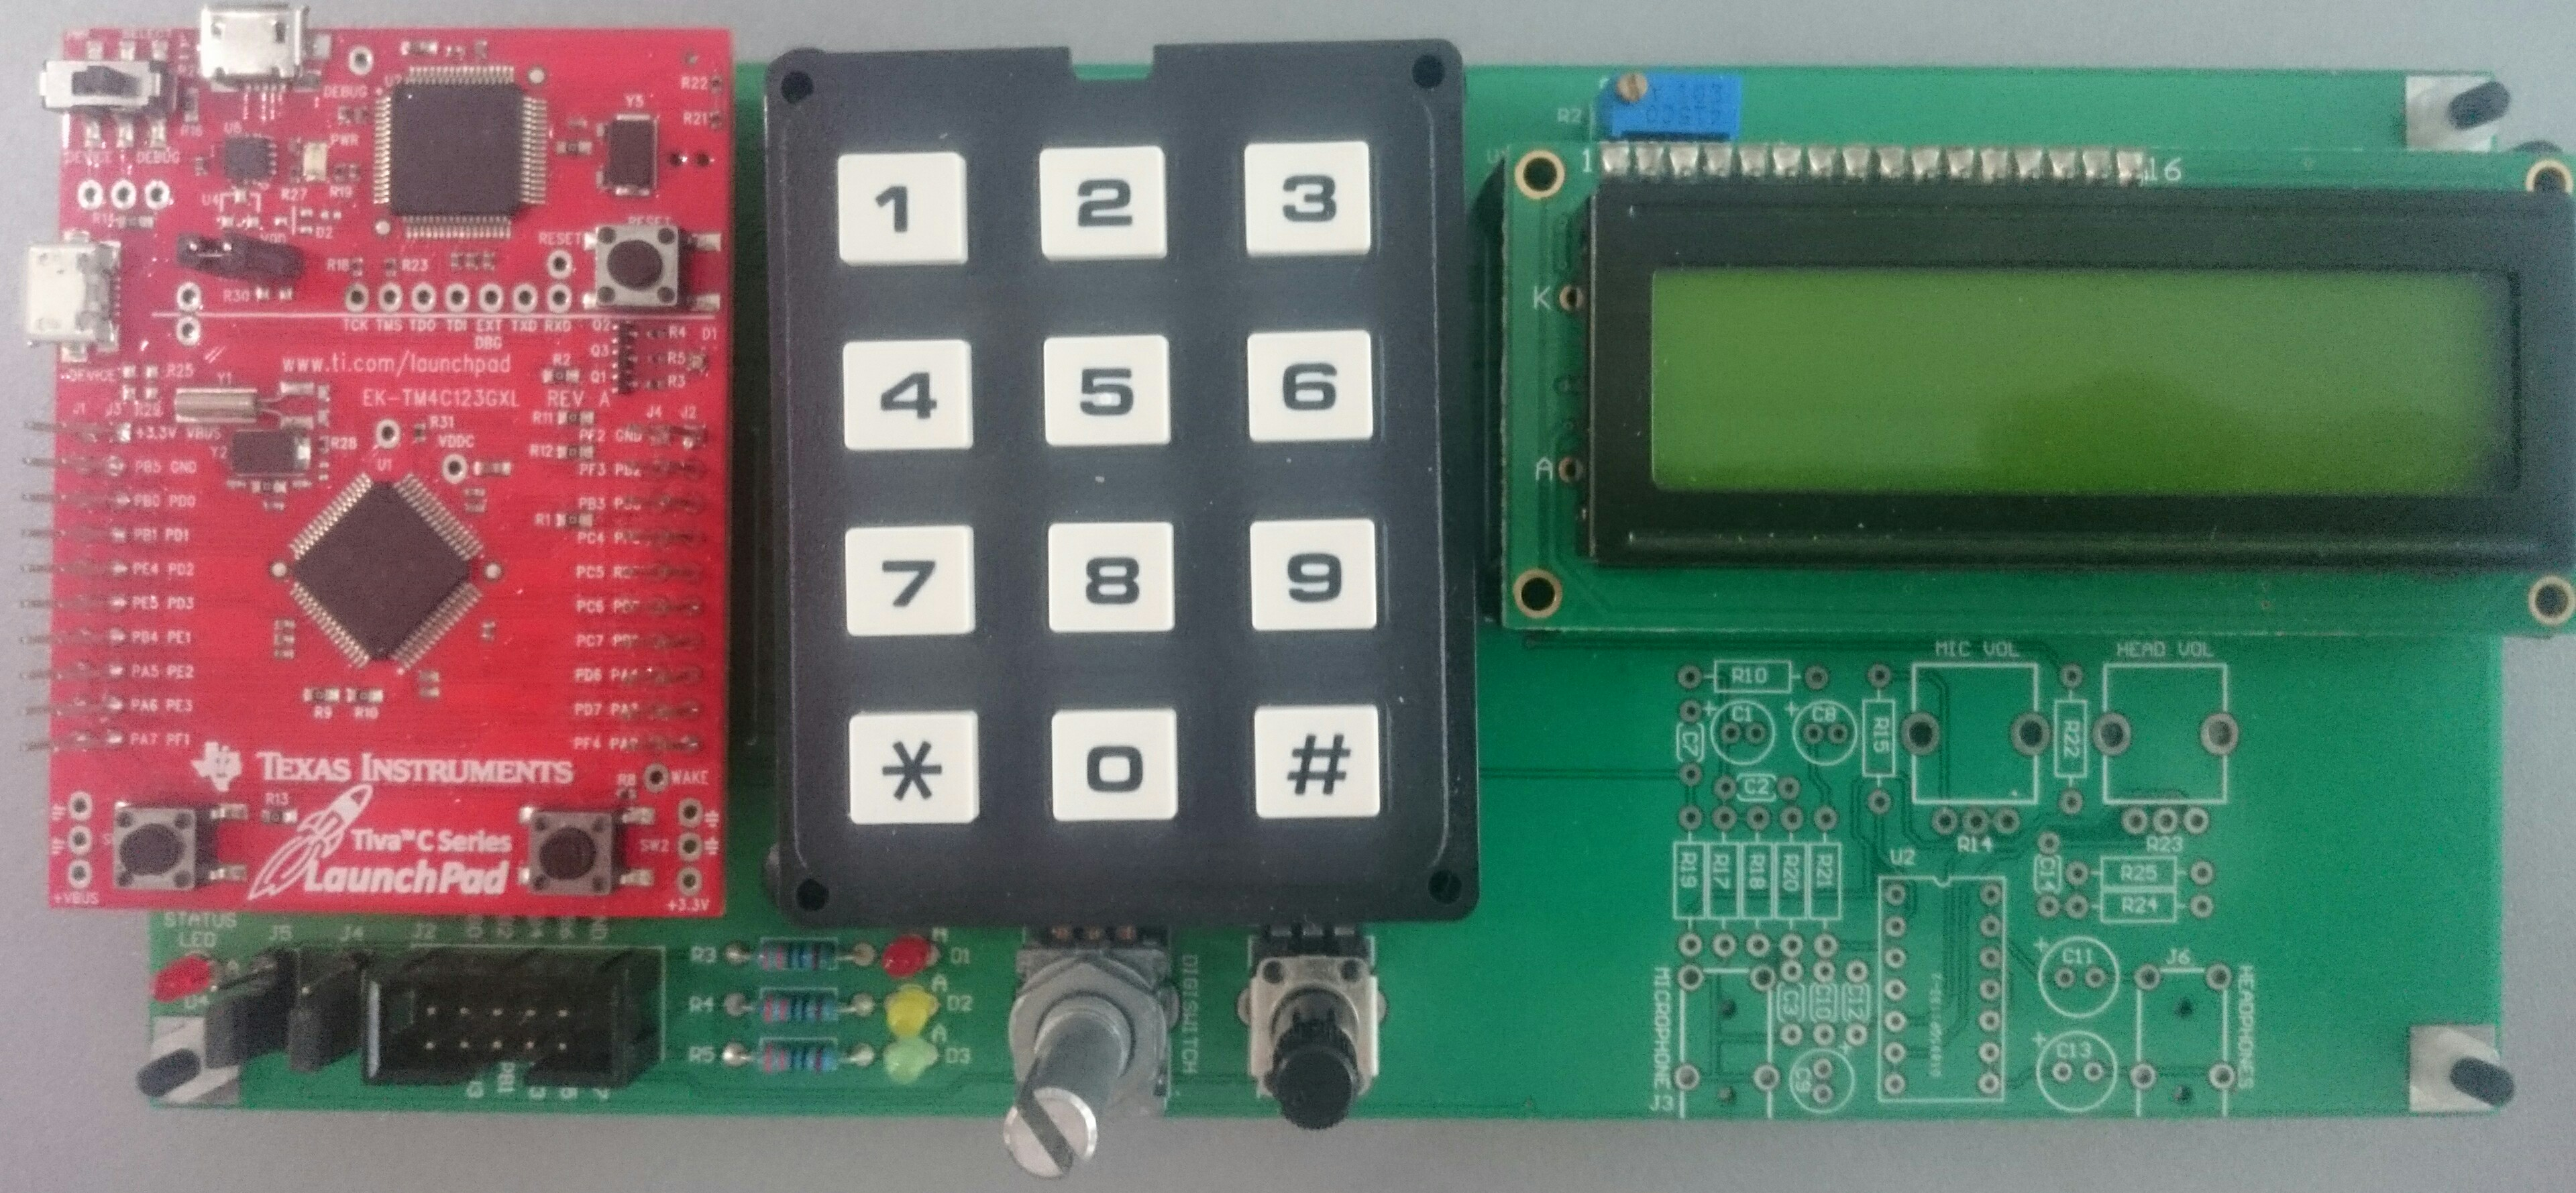
\includegraphics[scale=0.1, angle =0]{Billeder/EMP_BOARD.JPG}
	\end{center}
\caption{EMP Board med det tilføjede Launch pad board}
\label{fig:EMP_BOARD}
\end{figure}

\subsection{Field Programmable Gate Array}

FPGA'en styrer motorerne med et Pulse-width modulation (PWM) signal som sendes til h-broerne som bestemmer hvilken retning strømmen skal sendes til motoren så de både kan køre med og mod uret.


%Besskrive hvorfra vi år koordinatsættet (hvor på nettet)